
\documentclass{article}

\usepackage{fancyheadings}
\usepackage{amsmath}
\usepackage{amsfonts}
\usepackage{amssymb}
\usepackage{epsfig}
\usepackage{graphicx}
%\usepackage{doublespace}

\usepackage{KenChuArticleStyle}

%%%%%%%%%%%%%%%%%%%%%%%%%%%%%%%%%%%%%%%%%%%%%%
%%%%%%%%%%%%%%%%%%%%%%%%%%%%%%%%%%%%%%%%%%%%%%
%%%%%%%%%%%%%%%%%%%%%%%%%%%%%%%%%%%%%%%%%%%%%%
%%%%%%%%%%%%%%%%%%%%%%%%%%%%%%%%%%%%%%%%%%%%%%
%%%%%%%%%%%%%%%%%%%%%%%%%%%%%%%%%%%%%%%%%%%%%%

\begin{document}

%%%%%%%%%%%%%%%%%%%%%%%%%%%%%%%%%%%%%%%%%%%%%%

%\setcounter{page}{1}

\pagestyle{fancy}

%\input{../CourseSemesterUnique}

%\rhead[\CourseSemesterUnique]{Kenneth Chu (300517641)}
%\lhead[Kenneth Chu (300517641)]{\CourseSemesterUnique}
\rhead[Study Notes]{Kenneth Chu (300517641)}
\lhead[Kenneth Chu (300517641)]{Study Notes}
\chead[]{{\Large\bf Hypothesis Testing} \\
\vskip 0.1cm \normalsize \today}
\lfoot[]{}
\cfoot[]{}
\rfoot[]{\thepage}

%%%%%%%%%%%%%%%%%%%%%%%%%%%%%%%%%%%%%%%%%%%%%%

          %%%%% ~~~~~~~~~~~~~~~~~~~~ %%%%%

\section{Reminder: $\chi^{2}_{n}$ \;$=$\; ``sum of squares of $n$ independent standard-normals"}
\setcounter{theorem}{0}

Let $Z_{1}, Z_{2}, \ldots, Z_{n}$ be $n$ independent random variables with the standard normal distribution $\mathcal{N}(0,1)$.  Then,
$X_{n} := Z_{1}^{2} + Z_{2}^{2} + \cdots + Z_{n}^{2}$ has the $\chi^{2}_{n}$ distribution, the Chi-square distribution of $n$ degrees of freedom.

The probability density function of $X_{n}$ is given by:
\begin{equation*}
f_{X_{n}}(x) \; = \; \dfrac{1}{2^{n/2}\,\Gamma\!\left(\dfrac{n}{2}\right)} \; x^{(n/2)-1} \; e^{-x/2}\,,
\quad\textnormal{for}\;\; x \geq 0.
\end{equation*}

\begin{remark}\mbox{}\\
Note that
\begin{equation*}
          f_{\chi^{2}_{1}}(x)
\; = \; \dfrac{1}{2^{1/2}\,\Gamma\!\left(\dfrac{1}{2}\right)} \; x^{(1/2)-1} \; e^{-x/2}
\; = \; \dfrac{1}{\sqrt{2}\,\sqrt{\pi}}\;\,x^{-1/2} \; e^{-x/2}
\; = \; \dfrac{1}{\sqrt{2\pi} \cdot x^{1/2} \cdot e^{x/2}}
\end{equation*}
has a singularity at $x=0$, and
\begin{equation*}
          f_{\chi^{2}_{2}}(x)
\; = \; \dfrac{1}{2^{2/2}\,\Gamma\!\left(\dfrac{2}{2}\right)} \; x^{(2/2)-1} \; e^{-x/2}
\; = \; \dfrac{1}{{2}\;\Gamma\!\left(1\right)}\;x^{0} \; e^{-x/2}
\; = \; \dfrac{1}{2}\,e^{-x/2}
\end{equation*}
is simply an exponential decay in $x \geq 0$.
\end{remark}

The diagram below shows graphs of the probability density functions $f_{\chi^{2}_{1}}, \ldots, f_{\chi^{2}_{5}}$.
It is generated with \texttt{R} with the following commands:
\vskip 0.2cm
\texttt{
\small
\noindent\mbox{}\\
> x<-seq(0,10,0.001);  \\
> y1<-dchisq(x,df=1); y2<-dchisq(x,df=2); y3<-dchisq(x,df=3); y4<-dchisq(x,df=4); y5<-dchisq(x,df=5); \\
> plot(x,y1,ylim=c(0,0.6),type="l");
> points(x,y2,type="l",col="blue"); points(x,y3,type="l",col="green"); \\
> points(x,y4,type="l",col="red");points(x,y5,type="l",col="cyan"); \\
> legend("topright",c("df=1","df=2","df=3","df=4","df=5"),text.col=c("black","blue","green","red","cyan"));}
\mbox{}
\begin{center}
\vskip -1.0cm
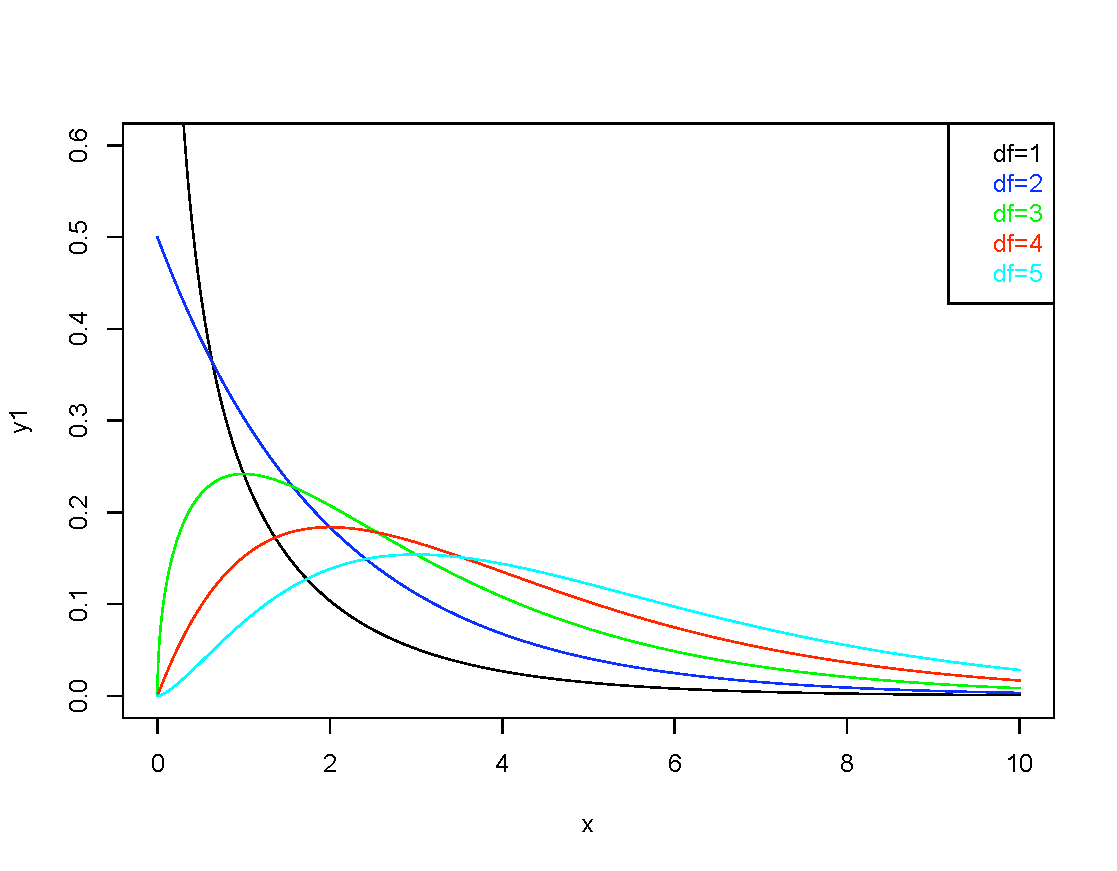
\includegraphics[height=10cm,width=14cm]{ChiSquare-df1-thru-df5.pdf}
\end{center}

          %%%%% ~~~~~~~~~~~~~~~~~~~~ %%%%%

\section{Reminder: $t_{n}$ \;$=$\; ``would-have-been standard-normal except for the estimated standard-deviation denominator"}\label{tDistribution}
\setcounter{theorem}{0}

\begin{itemize}
\item  Let $X_{1}, X_{2}, \ldots, X_{n}$ be \emph{i.i.d.} normal random variables
          with common mean $\mu$ and finite variance $\sigma^{2} > 0$.
          \begin{equation*}
          \overline{X}_{n} \; := \; \dfrac{1}{n}\,\sum_{i=1}^{n}X_{i}\,,
          \quad\quad\textnormal{and}\quad\quad
          S_{n}^{2} \; := \; \dfrac{1}{n-1}\,\sum_{i=1}^{n}\,\left(X_{i}-\overline{X}_{n}\right)^{2}.
          \end{equation*}
          $\overline{X}_{n}$ is called the \textbf{\emph{sample mean}}, and $S_{n}^{2}$ is called the
          (\textbf{\emph{unbiased}}) \textbf{\emph{sample variance}}.
          They are random variables and are unbiased estimators for $\mu$ and $\sigma^{2}$, respectively.
\item  Note that
          \begin{equation*}
          T_{n-1}
          \;\;:=\;\; \dfrac{\overline{X}_{n} - \mu}{\sqrt{S_{n}^{2}\,/\,n}}
          \;\; =\;\; \dfrac{\dfrac{\overline{X}_{n}-\mu}{\sigma/\sqrt{n}}}
                      {\sqrt{\left.\left(\dfrac{(n-1)\,S_{n}^{2}}{\sigma^{2}}\right)\right/(n-1)}}.
          \end{equation*}
          We claim:
          \begin{itemize}
          \item  The numerator $\dfrac{\overline{X}_{n}-\mu}{\sigma/\sqrt{n}}$ of $T_{n-1}$
                    has the standard normal distribution.
          \item  The term $\dfrac{(n-1)\,S_{n}^{2}}{\sigma^{2}}$ $=$
                    $\underset{i=1}{\overset{n}{\textnormal{\Large$\sum$}}}\left(\dfrac{X_{i}-\overline{X}_{n}}{\sigma}\right)^{2}$
                    in the denominator of $T_{n-1}$
                    is a random variable whose distribution is a $\chi^{2}$ distribution
                    with $(n-1)$ degrees of freedom.
          \item  The two random  variables $\dfrac{\overline{X}_{n}-\mu}{\sigma/\sqrt{n}}$ and
                    $\dfrac{(n-1)\,S_{n}^{2}}{\sigma^{2}}$ are independent of each other.
          \end{itemize}
\item  \begin{definition}\mbox{}\\
          Let $Z$ be a standard normal random variable and
          $X$ be a $\chi^{2}$ random variable with $n$ degrees of freedom.
          Suppse $Z$ and $X$ are independent.
          The \textbf{Student $t$ distribution with $n$ degrees of freedom} is the probability distribution of the following
          random variable:
          \begin{equation*}
          T_{n} \; := \; \dfrac{Z}{\sqrt{X/n}}.
          \end{equation*}
          The random variable $T_{n}$ is called the \textbf{Student's $t$ ratio with $n$ degrees of freedom}.
          \end{definition}
\item  \begin{theorem}\mbox{}\\
          The probability density function of the Student $t$ distribution with $n$ degrees of freedom is given by:
          \begin{equation*}
          f_{T_{n}}(t) \; = \; \dfrac{\Gamma\!\left(\dfrac{n+1}{2}\right)}{\sqrt{n\,\pi}\,\Gamma\!\left(\dfrac{n}{2}\right)}
                                      \cdot
                                      \dfrac{1}{\left(1+\dfrac{t^{2}}{n}\right)^{(n+1)/2}}\,,
          \quad\textnormal{for}\;\; -\infty < t < \infty.
          \end{equation*}
          \end{theorem}
\end{itemize}

The diagram below shows the graphs of the probability density functions $f_{T_{20}}$ in black and $f_{T_{2}}$ in red.
\begin{center}
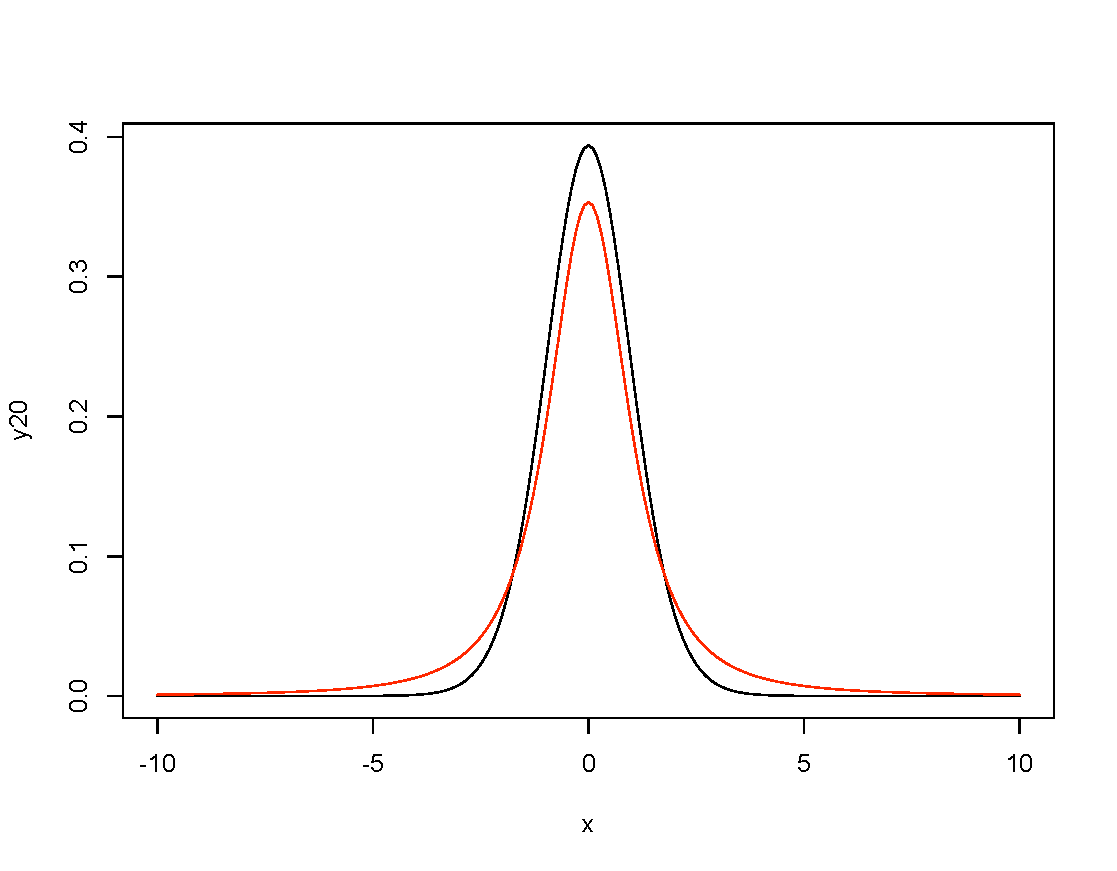
\includegraphics[height=10cm,width=14cm]{StudentTDist-df20-df2.pdf}
\end{center}
The above graph is generated with \texttt{R} with the following command:
\begin{center}
\texttt{> y20 = dt(x,df=20); y2 = dt(x,df=2); plot(x,y20,type="l"); points(x,y2,type="l",col="red");}
\end{center}

          %%%%% ~~~~~~~~~~~~~~~~~~~~ %%%%%

\section{Reminder: $\mathcal{F}^{m}_{n}$ \;$=$\; ``ratio of two independent $\chi^{2}$ random variables"}
\setcounter{theorem}{0}

\begin{definition}\mbox{}\\
Let $m,n \in \N$.  Let $X_{m} \sim \chi^{2}_{m}$ and $X_{n} \sim \chi^{2}_{n}$ be independent $\chi^{2}$ random variables with the indicated degrees of freedom.  For $m, n \in \N$, the \textbf{F distribution with $m$ and $n$ degrees of freedom}, denoted by $\mathcal{F}^{m}_{n}$, is the probability distribution of the following random variable:
\begin{equation*}
F := \dfrac{X_{m}/m}{X_{n}/n}.
\end{equation*}
\end{definition}

\begin{theorem}\label{pdf:Fmn}\mbox{}\\
The probability density function of the F distribution $\mathcal{F}^{m}_{n}$ with $m$ and $n$ degrees of freedom is given by:
\begin{equation*}
         f_{\mathcal{F}^{m}_{n}}\!\left(\zeta\right)
\; = \; \left(
         m^{m/2} \cdot n^{n/2}\cdot
         \dfrac{\Gamma\!\left(\frac{m+n}{2}\right)}{\Gamma\!\left(\frac{m}{2}\right)\,\Gamma\!\left(\frac{n}{2}\right)}
         \right)\cdot
         \dfrac{\zeta^{(m/2)-1}}{(m\,\zeta + n)^{(m+n)/2}},
\quad\textnormal{for}\;\; \zeta \geq 0.
\end{equation*}
\end{theorem}

\begin{remark}\mbox{}\\
The ``F'' in ``F distribution'' commemorates the renowned statistician Sir Ronald Fisher. \vskip 0.1cm

\noindent
Let $T = \dfrac{Z}{\sqrt{X/n}}$ be a Student $t$ ratio, i.e. $Z$ and $X$ are independent random variables with $Z \sim \mathcal{N}(0,1)$ and $X \sim \chi^{2}_{n}$.  Then, $Z^{2} \sim \chi^{2}_{1}$.  Hence, $T^{2} = \dfrac{Z^{2}}{X/n} = \dfrac{Z^{2}/1}{X/n} \sim \mathcal{F}^{1}_{n}$, the F distribution with $m=1$ and $n$ degrees of freedom. 
%We will derive the probability density function for the distribution of $T$ by using that of $T^{2}$ as given by Theorem \ref{pdf:Fmn}.
\end{remark}

          %%%%% ~~~~~~~~~~~~~~~~~~~~ %%%%%

\section{Testing: $H_{0} : \mu = \mu_{0}$ --- the one-sample $t$-test for a normal distribution with unknown mean $\mu$}
\setcounter{theorem}{0}

See \S\ref{tDistribution}.

          %%%%% ~~~~~~~~~~~~~~~~~~~~ %%%%%

\section{Testing: $H_{0} : \mu_{X} = \mu_{Y}$ --- the two-sample $t$-test for two normal distributions with unknown means $\mu_{X}$ and $\mu_{Y}$ but equal (but no-need-to-be-known) variances}
\setcounter{theorem}{0}

Suppose $X_{1},\ldots,X_{n},Y_{1},\ldots,Y_{m}$ are independent random variables.  Suppose also $X_{1},\ldots,X_{n} \sim \mathcal{N}(\mu_{X},\sigma^{2}_{X})$, and $Y_{1},\ldots,Y_{m} \sim \mathcal{N}(\mu_{Y},\sigma^{2}_{Y})$.

Then, $\textnormal{Var}\!\left(\,\overline{X}-\overline{Y}\,\right)$
$=$ $\textnormal{Var}\!\left(\,\overline{X}\,\right) + \textnormal{Var}\!\left(\,\overline{Y}\,\right)$
$=$ $\dfrac{1}{n}\textnormal{Var}\!\left(X\right) + \dfrac{1}{m}\textnormal{Var}\!\left(Y\right)$
$=$ $\dfrac{\sigma^{2}_{X}}{n} + \dfrac{\sigma^{2}_{Y}}{m}$.  Hence,
\begin{equation*}
\dfrac{\overline{X}-\overline{Y} - \left(\mu_{X}-\mu_{Y}\right)}{\sqrt{\dfrac{\sigma^{2}_{X}}{n} + \dfrac{\sigma^{2}_{Y}}{m}}}
\quad\sim\quad\mathcal{N}(0,1).
\end{equation*}
And,
\begin{equation*}
  \sum^{n}_{i=1}\left(\dfrac{X_{i}-\overline{X}}{\sigma_{X}}\right)^{2}
+\sum^{m}_{i=1}\left(\dfrac{Y_{i}-\overline{Y}}{\sigma_{Y}}\right)^{2}
\quad\sim\quad
\chi^{2}_{n-1+m-1} \; = \; \chi^{2}_{n+m-2} 
\end{equation*}
Hence,
\begin{equation*}
\dfrac{
\dfrac{\overline{X}-\overline{Y} - \left(\mu_{X}-\mu_{Y}\right)}{\sqrt{\dfrac{\sigma^{2}_{X}}{n} + \dfrac{\sigma^{2}_{Y}}{m}}}
}
{
\left(
\dfrac{1}{n+m-2}
\left\{
  \underset{i=1}{\overset{n}{\textnormal{\large$\sum$}}}\left(\dfrac{X_{i}-\overline{X}}{\sigma_{X}}\right)^{2}
+\underset{i=1}{\overset{m}{\textnormal{\large$\sum$}}}\left(\dfrac{Y_{i}-\overline{Y}}{\sigma_{Y}}\right)^{2}
\right\}
\right)^{1/2}
}
\quad\sim\quad t_{n+m-2} 
\end{equation*}
Now, \textbf{\large suppose further $\sigma^{2}_{X} = \sigma^{2}_{Y}$}.  Then,
\begin{equation*}
H_{0} \,:\, \mu_{X} = \mu_{Y}
\quad\Longrightarrow\quad
%\left(
\dfrac{1}{\sqrt{\dfrac{1}{n} + \dfrac{1}{m}}} \cdot
%\right)
\dfrac{
\overline{X}-\overline{Y}
}
{
\left(
\dfrac{1}{n+m-2}
\left\{
  \underset{i=1}{\overset{n}{\textnormal{\large$\sum$}}}\left(X_{i}-\overline{X}\right)^{2}
+\underset{i=1}{\overset{m}{\textnormal{\large$\sum$}}}\left(Y_{i}-\overline{Y}\right)^{2}
\right\}
\right)^{1/2}
}
\quad\sim\quad t_{n+m-2} 
\end{equation*}

          %%%%% ~~~~~~~~~~~~~~~~~~~~ %%%%%

\section{Testing: $H_{0} : \mu_{1} = \mu_{2} = \cdots = \mu_{k}$ --- the $F$-test and ANOVA (analysis of variance)}
\setcounter{theorem}{0}

Suppose we are given $k \in \N$, and $n_{1},n_{2},\ldots,n_{k} \in\N$.  Let $n := n_{1} + \cdots + n_{k}$.
Suppose further we are given a doubly indexed set of \textbf{independent} random variables
\begin{equation*}
\left\{\; \left. Y_{ij} \;\right\vert\;  1 \leq i \leq k, 1 \leq j \leq n_{i} \;\right\}.
\end{equation*}
Suppose that each $Y_{ij}$ has the form:
\begin{equation*}
    Y_{ij} \; = \; \mu_{i} + \epsilon_{ij},
\end{equation*}
where $\mu_{i} \in \Re$ is constant, and $\epsilon_{ij} \sim \mathcal{N}(0,\sigma^{2})$.
The \emph{between-cluster sum of squares} SSB and the \emph{within-cluster sum of squares} SSW are defined as follows:
\begin{eqnarray*}
\textnormal{SSB} & := &
\sum^{k}_{i=1}\sum^{n_{i}}_{j=1}\left(\,\overline{Y}_{i}-\overline{Y}\,\right)^{2}
\;\;=\;\;
\sum^{k}_{i=1}\,n_{i}\left(\,\overline{Y}_{i}-\overline{Y}\,\right)^{2} \,, \\
\textnormal{SSW} & := &
\sum^{k}_{i=1}\sum^{n_{i}}_{j=1}\left(\,Y_{ij} - \overline{Y}_{i}\,\right)^{2}\,,
\end{eqnarray*}
where
\begin{equation*}
\overline{Y}_{i} \; := \; \dfrac{1}{n_{i}}\sum^{n_{i}}_{j=1}Y_{ij}\,,
\quad
\overline{Y} \; := \; \dfrac{1}{n}\sum^{k}_{i=1}\sum^{n_{i}}_{j=1}Y_{ij} \; = \; \dfrac{1}{n}\sum^{k}_{i=1}n_{i}\,\overline{Y}_{i} \,.
\end{equation*}
Note that
\begin{equation*}
\dfrac{\textnormal{SSW}}{\sigma^{2}} \; := \;
\sum^{k}_{i=1}\sum^{n_{i}}_{j=1}\left(\,\dfrac{Y_{ij} - \overline{Y}_{i}}{\sigma}\,\right)^{2}
\end{equation*}
has a $\chi^{2}$ distribution of $\sum^{k}_{i=1}(n_{i}-1) = n - k$ degrees of freedom.
\begin{theorem}\quad
SSB and SSW are independent random variables.
\end{theorem}
\begin{theorem}\quad
If $\mu_{1} = \mu_{2} = \cdots = \mu_{k}$, then
\begin{itemize}
    \item  $\dfrac{\textnormal{SSB}}{\sigma^{2}}$ has a $\chi^{2}$ distribution of $k-1$ degrees of freedom.
              \begin{equation*}
                   \dfrac{\textnormal{SSB}}{\sigma^{2}}
                   \; = \;
                   \dfrac{1}{\sigma^{2}}\,\sum^{k}_{i=1}\,n_{i}\left(\,\overline{Y}_{i}-\overline{Y}\,\right)^{2}
                   \; = \;
                   \sum^{k}_{i=1} \, \dfrac{1}{\sigma^{2}/n_{i}} \left(\,\overline{Y}_{i}-\overline{Y}\,\right)^{2}
                   \; = \;
                   \sum^{k}_{i=1} \left(\,\dfrac{\overline{Y}_{i}-\overline{Y}}{\sigma/\sqrt{n_{i}}}\,\right)^{2}
              \end{equation*}
    \item  Consequently,
              \begin{equation*}
                  \dfrac{SSB/(k-1)}{SSW/(n-k)}
                  \; = \;
                  \dfrac{
                      \dfrac{1}{k-1}\,
                      \underset{i=1}{\overset{k}{\textnormal{\large$\sum$}}}\,
                      n_{i}\left(\,\overline{Y}_{i}-\overline{Y}\,\right)^{2}
                  }{
                      \dfrac{1}{n-k}\,
                      \underset{i=1}{\overset{k}{\textnormal{\large$\sum$}}}\,
                      \underset{j=1}{\overset{n_{i}}{\textnormal{\large$\sum$}}}
                      \left(\,Y_{ij} - \overline{Y}_{i}\,\right)^{2}
                  }
                  \; \sim \; \mathcal{F}^{k-1}_{n-k}
              \end{equation*}
\end{itemize}
\end{theorem}

          %%%%% ~~~~~~~~~~~~~~~~~~~~ %%%%%

\section{Testing: $H_{0} : \sigma^{2}_{X} = \sigma^{2}_{Y}$ --- the (two-sample) $F$-test for two normal distributions}
\setcounter{theorem}{0}

Suppose $X_{1},\ldots,X_{n},Y_{1},\ldots,Y_{m}$ are independent random variables.  Suppose also $X_{1},\ldots,X_{n} \sim \mathcal{N}(\mu_{X},\sigma^{2}_{X})$, and $Y_{1},\ldots,Y_{m} \sim \mathcal{N}(\mu_{Y},\sigma^{2}_{Y})$.

Let
\begin{equation*}
    S^{2}_{X} \;:=\; \dfrac{1}{n-1}\,\sum^{n}_{i=1}\left(X_{i}-\overline{X}\right)^{2}
    \quad\textnormal{and}\quad
    S^{2}_{Y} \;:=\; \dfrac{1}{m-1}\,\sum^{m}_{i=1}\left(Y_{i}-\overline{Y}\right)^{2}.
\end{equation*}
Recall that
\begin{equation*}
    \dfrac{(n-1)S^{2}_{X}}{\sigma^{2}_{X}} \;=\; \dfrac{1}{\sigma^{2}_{X}}\,\sum^{n}_{i=1}\left(X_{i}-\overline{X}\right)^{2}\;\sim\;\chi^{2}_{n-1}
    \quad\textnormal{and}\quad
    \dfrac{(m-1)S^{2}_{Y}}{\sigma^{2}_{Y}} \;=\; \dfrac{1}{\sigma^{2}_{Y}}\,\sum^{m}_{i=1}\left(Y_{i}-\overline{Y}\right)^{2}\;\sim\;\chi^{2}_{m-1}.
\end{equation*}
Consequently,
\begin{equation*}
   \dfrac{S^{2}_{Y}/\sigma^{2}_{Y}}{S^{2}_{X}/\sigma^{2}_{X}}
   \;=\;
   \dfrac{\left.\frac{1}{m-1}\sum^{m}_{j=1}\left(Y_{j}-\overline{Y}\right)^{2}\right/\sigma^{2}_{Y}}
            {\left.\frac{1}{n-1}\sum^{n}_{i=1}\left(X_{i}-\overline{X}\right)^{2}\right/\sigma^{2}_{X}}
    \;\;\sim\;\;
    \mathcal{F}^{m-1}_{n-1}
\end{equation*}
Therefore,
\begin{equation*}
   H_{0}\,:\,\sigma^{2}_{X} = \sigma^{2}_{Y}
   \quad\Longrightarrow\quad
   \dfrac{S^{2}_{Y}}{S^{2}_{X}}
   \;=\;\dfrac{\frac{1}{m-1}\sum^{m}_{j=1}\left(Y_{j}-\overline{Y}\right)^{2}}
            {\frac{1}{n-1}\sum^{n}_{i=1}\left(X_{i}-\overline{X}\right)^{2}}
    \;\;\sim\;\;
    \mathcal{F}^{m-1}_{n-1}
\end{equation*}


          %%%%% ~~~~~~~~~~~~~~~~~~~~ %%%%%

\section{$\chi^{2}$ Goodness-of-fit test --- testing goodness-of-fit of a probability model via an induced multinomial model}
\setcounter{theorem}{0}

Suppose $\mathbf{X} = \left(\,X_{1},X_{2},\ldots,X_{k}\,\right)$ has a multinomial distribution with number-of-trials parameter $n$ and probability parameter $\mathbf{p} = (p_{1},p_{2},\ldots,p_{k})$, with $p_{i}>0$, for each $i=1,2,\ldots,k$.  In other words, $\mathbf{X} \sim \textnormal{Multinomial}(n,\mathbf{p})$, or equivalently, $(X_{1},X_{2},\ldots,X_{k}) \sim \textnormal{Multinomial}(n,(p_{1},p_{2},\ldots,p_{k}))$.  This simply means:
\begin{equation*}
  \textnormal{Prob}\!\left(\,X_{1}=m_{1},\,X_{2}=m_{2},\,\ldots,\,X_{k}=m_{k}\,\right)
  \; = \;
  \dfrac{n!}{m_{1}!\,m_{2}!\,\cdots\,m_{k}!}\;p_{1}^{m_{1}}\,p_{2}^{m_{2}}\,\cdots\,p_{k}^{m_{k}}.
\end{equation*}
Note that the random variables $X_{1}, X_{2}, \ldots, X_{k}$ are subject to the restriction: $\sum_{i=1}^{k}X_{i} = n$.

\begin{theorem}\quad
The random variable
\begin{equation*}
   D \; := \;
   \sum^{k}_{i=1}\, \dfrac{(X_{i}-n\,p_{i})^{2}}{n\,p_{i}}
\end{equation*}
has \textbf{approximately} a $\chi^{2}_{k-1}$ distribution.\\
(That the degree of freedom is $k-1$, rather than $k$, is a manifestation of the restriction that $\sum_{i=1}^{k}X_{i} = n$.)
\end{theorem}

Suppose $\mathbf{X} = \left(\,X_{1},X_{2},\ldots,X_{k}\,\right)$ has a multinomial distribution with number-of-trials parameter $n$ and probability parameter $\mathbf{p}(\Theta) = (p_{1}(\Theta),p_{2}(\Theta),\ldots,p_{k}(\Theta))$, with $p_{i}(\Theta)>0$, for each $i=1,2,\ldots,k$, where $\Theta = (\theta_{1},\theta_{2},\ldots,\theta_{s}) \in \Re^{s}$ is a vector parameter of the multinomial model.
Let $\widehat{p}_{1}:= p_{1}\!\left(\widehat{\Theta}_{\textnormal{MLE}}\right)$, $\widehat{p}_{2}:= p_{2}\!\left(\widehat{\Theta}_{\textnormal{MLE}}\right)$, $\ldots,$ $\widehat{p}_{k}:= p_{k}\!\left(\widehat{\Theta}_{\textnormal{MLE}}\right)$.

\begin{theorem}\quad
The random variable
\begin{equation*}
   D_{1} \; := \;
   \sum^{k}_{i=1}\, \dfrac{(X_{i}-n\,\widehat{p}_{i})^{2}}{n\,\widehat{p}_{i}}
\end{equation*}
has \textbf{approximately} a $\chi^{2}_{k-s-1}$ distribution.
\end{theorem}

          %%%%% ~~~~~~~~~~~~~~~~~~~~ %%%%%

%%%%%%%%%%%%%%%%%%%%%%%%%%%%%%%%%%%%%%%%%%%%%%

\appendix

          %%%%% ~~~~~~~~~~~~~~~~~~~~ %%%%%

%%%%%%%%%%%%%%%%%%%%%%%%%%%%%%%%%%%%%%%%%%%%%%

%\bibliographystyle{alpha}
%\bibliographystyle{plain}
%\bibliographystyle{amsplain}
\bibliographystyle{acm}
\bibliography{KenChuBioinformatics}

%%%%%%%%%%%%%%%%%%%%%%%%%%%%%%%%%%%%%%%%%%%%%%
%%%%%%%%%%%%%%%%%%%%%%%%%%%%%%%%%%%%%%%%%%%%%%
%%%%%%%%%%%%%%%%%%%%%%%%%%%%%%%%%%%%%%%%%%%%%%
%%%%%%%%%%%%%%%%%%%%%%%%%%%%%%%%%%%%%%%%%%%%%%
%%%%%%%%%%%%%%%%%%%%%%%%%%%%%%%%%%%%%%%%%%%%%%

\end{document}

